% Byte range diagram: trailing bytes attack (Chapter 13)
\documentclass[border=10pt]{standalone}
\usepackage{tikz}
\usetikzlibrary{positioning, decorations.pathreplacing, calc}
\usepackage{fontspec}
\setmainfont{Noto Serif}
\setsansfont{Noto Sans}
\setmonofont{DejaVu Sans Mono}[Scale=0.85]
\usepackage{xcolor}
\definecolor{signed}{HTML}{c8e6c9}
\definecolor{gap}{HTML}{ffcdd2}
\definecolor{malicious}{HTML}{ff8a80}
\definecolor{accent}{HTML}{0f3460}

\begin{document}
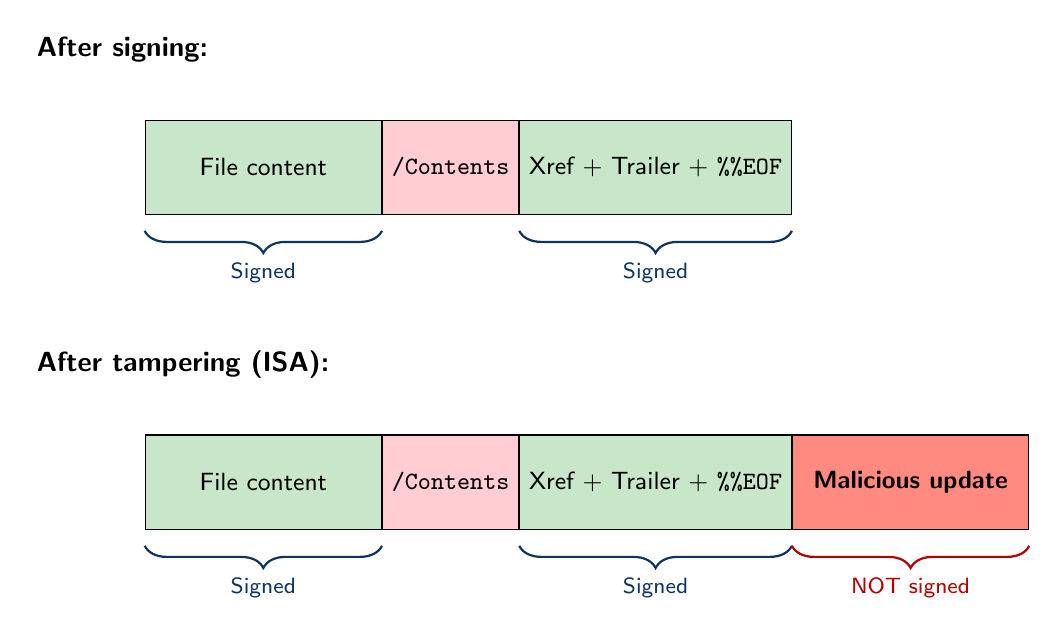
\begin{tikzpicture}[
    block/.style={draw, minimum height=1.2cm, text centered, font=\sffamily\small},
    brace/.style={decorate, decoration={brace, amplitude=8pt, mirror}},
]

% Row 1: After signing (valid)
\node[font=\sffamily\bfseries, anchor=west] (title1) at (0, 2) {After signing:};

\node[block, fill=signed, minimum width=3cm] (h1) at (3, 0.5) {File content};
\node[block, fill=gap, minimum width=1.5cm, right=0pt of h1] (c1) {\texttt{/Contents}};
\node[block, fill=signed, minimum width=3cm, right=0pt of c1] (x1) {Xref + Trailer + \texttt{\%\%EOF}};

\draw[brace, thick, accent] ($(h1.south west) + (0,-0.2)$) -- node[below=8pt, font=\sffamily\footnotesize, text=accent] {Signed} ($(h1.south east) + (0,-0.2)$);
\draw[brace, thick, accent] ($(x1.south west) + (0,-0.2)$) -- node[below=8pt, font=\sffamily\footnotesize, text=accent] {Signed} ($(x1.south east) + (0,-0.2)$);

% Row 2: After tampering
\node[font=\sffamily\bfseries, anchor=west] (title2) at (0, -2) {After tampering (ISA):};

\node[block, fill=signed, minimum width=3cm] (h2) at (3, -3.5) {File content};
\node[block, fill=gap, minimum width=1.5cm, right=0pt of h2] (c2) {\texttt{/Contents}};
\node[block, fill=signed, minimum width=3cm, right=0pt of c2] (x2) {Xref + Trailer + \texttt{\%\%EOF}};
\node[block, fill=malicious, minimum width=3cm, right=0pt of x2, font=\sffamily\small\bfseries] (mal) {Malicious update};

\draw[brace, thick, accent] ($(h2.south west) + (0,-0.2)$) -- node[below=8pt, font=\sffamily\footnotesize, text=accent] {Signed} ($(h2.south east) + (0,-0.2)$);
\draw[brace, thick, accent] ($(x2.south west) + (0,-0.2)$) -- node[below=8pt, font=\sffamily\footnotesize, text=accent] {Signed} ($(x2.south east) + (0,-0.2)$);
\draw[brace, thick, red!70!black] ($(mal.south west) + (0,-0.2)$) -- node[below=8pt, font=\sffamily\footnotesize, text=red!70!black] {NOT signed} ($(mal.south east) + (0,-0.2)$);

\end{tikzpicture}
\end{document}
